\chapter{Introduction}

% the code below specifies where the figures are stored
\ifpdf
    \graphicspath{{1_introduction/figures/PNG/}{1_introduction/figures/PDF/}{1_introduction/figures/}}
\else
    \graphicspath{{1_introduction/figures/EPS/}{1_introduction/figures/}}
\fi

\section{Motivation and Problem Statement}

A~very open definition of the word \emph{event}
given by WordNet~\cite{Princeton:WordNet} is
\emph{``something that happens at a given place and time''}.
Following this definition,
we are indeed surrounded by events, most of them
are of little to no interest for us.
A~concert somewhere in the world of a~band
that we do not even know may be a~good example.
For some events, however, we may care more, for example,
a~concert of a~band that we know and like,
even if it takes place at a~location far away from us.
Finally, for very few events, we may care a~lot,
maybe even enough to physically attend the event,
like a~concert of our favorite band
if it takes place in our city, is not sold out,
and not too expensive.

All this motivates the need for \emph{event summarization}.
If there is an event that we could not attend
for a~reason whatsoever,
but that we are interested in,
a~good event summarization can help us get a~feeling
for the event's atmosphere.
Similarly, if there is an event that we attended,
we can revive the event's most fascinating moments
based on the event summarization.

A~\emph{media gallery} in the context of
our event summarization task is
a~compilation of images, videos,
and microposts retrieved from social networks
that are related to a~given event.
High quality media galleries have the following properties:

\begin{enumerate}
  \item \textit{Conciseness:}
        they convey a~lot of information clearly
        and in few media items.
  \item \textit{Comprehensiveness:}
        they are complete, including all representative
        elements or aspects of an event.
  \item \textit{Authenticity:}
        they are of undisputed origin and genuine.
  \item \textit{Diversity:}
        they show a~great deal of variety.
  \item \textit{Interestingness:}
        they catch and hold the attention of the viewer.     
\end{enumerate}

Event summarization covers textual,
as well as multimedia content.
For bigger events, official TV or newspaper journalists
report on site, and oftentimes the event organizers themselves
share official media material,
or even an official press package with event reports and images.

\section{Research Question and Hypothesis}
The main research question for this thesis
can be formulated as follows.
 
\noindent \textit{``Can user-customizable
media galleries that summarize given events be
created solely based on textual and multimedia data
from social networks?''}

\noindent The hypothesis that we test in this thesis
can be formulated as follows.

\noindent \textit{We argue that
through media galleries that leverage content
shared on social networks
a~more \emph{authentic}, more \emph{concise},
more \emph{comprehensive}, more \emph{diverse},
and also more \emph{interesting}
view on events gets possible than by limiting oneself
to officially produced media content;
and that further such media galleries can be generated
more \emph{efficiently} and \emph{in shorter time}
than the officially produced ones.}

\noindent We validate these subjective and objective
criteria with experiments for events of different categories
such as sports, politics, culture, leisure,
music, conferences, \emph{etc.}

\section{Approach}
\begin{figure}[htb!]
  \centering
  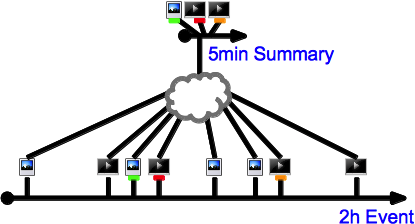
\includegraphics[width=0.45\textwidth]{thesis-diagram.png}
  \caption{Event summarization generation based on deduplicated, clustered, and ranked media items for an exemplary event, depicted in a~schematic manner.}     
  \label{fig:thesis-diagram}
\end{figure}

\section{Contributions}
\todo{add contributions as prose, "bragging rights"}

\section{The Web and Semantics}
Tim Berners Lee, inventor of the World-Wide Web (W3, WWW), or simply, the \emph{Web}, \emph{et al.}
write in~\cite{BernersLee1994}: \textit{``The World-Wide Web was developed
to be a pool of human knowledge, which would allow collaborators
in remote sites to share their ideas
and all aspects of a common project''}.
Since the earliest days at CERN,
the European Particle Physics Laboratory in Geneva, Switzerland,
the Web has scaled to a truly global system of interlinked hypertext documents
accessed via the Internet.

\emph{Semantics} is the study of meaning.
It focuses on the relation between signifiers, such as words, phrases, signs, and symbols,
and what they stand for, \emph{i.e.}, their denotata.
Michel Bréal is often identified as a~founder of modern semantics with his 1897
\emph{Essai de sémantique}~\cite{Breal1897}.
The \emph{Semantic Web} brings these two worlds together.

\section{Boundaries of this Work}

\section{Thesis Structure}